\section{Research questions}

%\section{Future work}

%%%%%%% Measurement approache
\begin{frame}[noframenumbering]
  \frametitle{Approach}
  \begin{itemize}
   \item Naxsi isolation (HTTP 200 OK)
     \begin{itemize}
       \item Baseline performance measurement
       \item Incrementing URL parameters
     \end{itemize}
   \item Real-life scenario (Wordpress)
     \begin{itemize}
       \item Baseline performance measurement
       \item Incrementing URL parameters
     \end{itemize}
  \end{itemize}
\end{frame}

%%%%%%% HTTP 200 OK: baseline performance measurement
\begin{frame}[noframenumbering]
  \frametitle{HTTP 200 OK: baseline performance measurement}
  \begin{figure}[H]
  \centering
  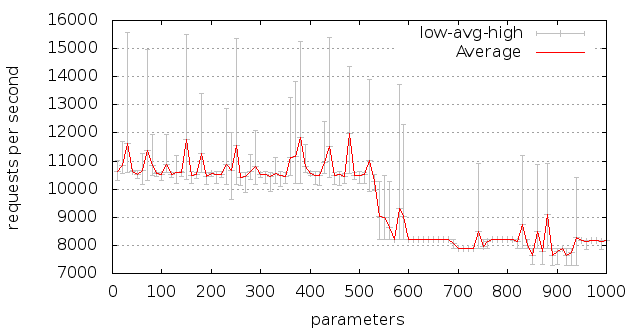
\includegraphics[scale=0.5] {../paper/images/results/baseline_200/output.png}
  \end{figure}
\end{frame}

%%%%%%% HTTP 200 OK: URL allowed paramter increments
\begin{frame}[noframenumbering]
  \frametitle{HTTP 200 OK: incrementing allowed URL parameters}

  \mbox{http://example.com/?foo1=bar1}\\
  \mbox{http://example.com/?foo1=bar1\&foo2=bar2}

  \begin{figure}[H]
  \centering
  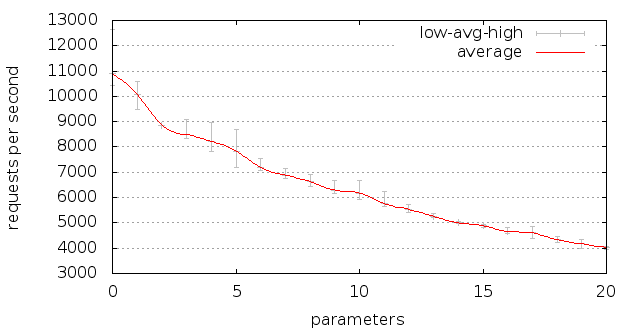
\includegraphics[scale=0.5] {../paper/images/results/200_with_naxsi_incremented_allowed_parameters/output.png}
  \end{figure}
\end{frame}

%%%%%%% HTTP 200 OK: URL disallowed paramter increments
\begin{frame}[noframenumbering]
  \mbox{http://example.com/?../}\\
  \mbox{http://example.com/?foo1=bar1\&../}

  \frametitle{HTTP 200 OK: incremting disallowed URL paramters}
  \begin{figure}[H]
  \centering
  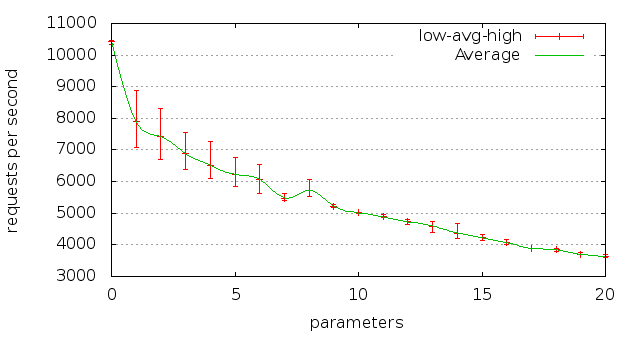
\includegraphics[scale=0.5] {../paper/images/results/200_with_naxsi_incremented_disallowed_parameters/output.png}
  \end{figure}
\end{frame}

%%%%%%% Wordpress baseline
\begin{frame}[noframenumbering]
  \frametitle{Wordpress: baseline performance measurement}
  \begin{figure}[H]
  \centering
  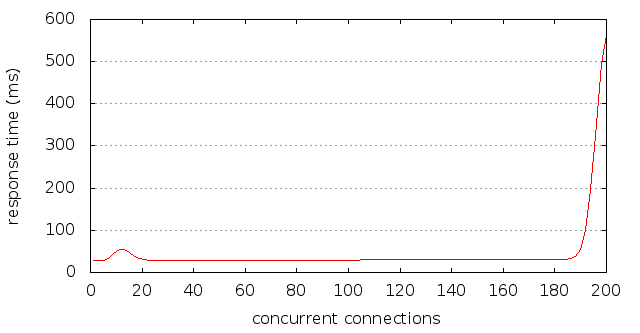
\includegraphics[scale=0.5] {../paper/images/results/baseline_wp/output.png}
  \end{figure}
\end{frame}

%%%%%%% Wordpress with Naxsi
\begin{frame}[noframenumbering]
  \mbox{http://example.com/?foo1=bar1}\\
  \mbox{http://example.com/?foo1=bar1\&foo2=bar2}

  \frametitle{Wordpress: incrementing allowed URL parameters}
  \begin{figure}[H]
  \centering
  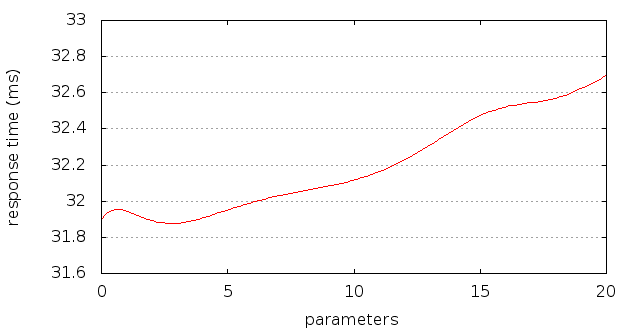
\includegraphics[scale=0.5] {../paper/images/results/wp_with_naxsi_incremented_allowed_parameters/output.png}
  \end{figure}
\end{frame}  
  
%%%%%%% Wordpress with Naxsi
\begin{frame}[noframenumbering]
  \mbox{http://example.com/?../}\\
  \mbox{http://example.com/?foo1=bar1\&../}
  
  \frametitle{Wordpress: incrementing disallowed URL parameters}
  \begin{figure}[H]
  \centering
  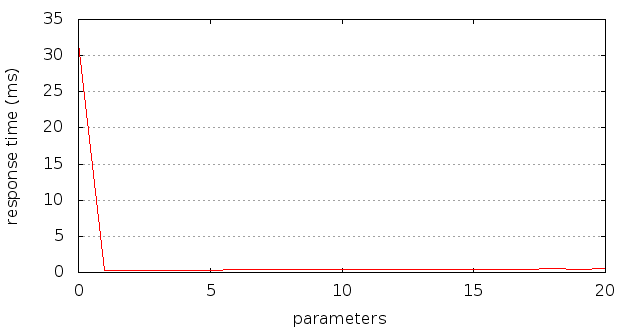
\includegraphics[scale=0.5] {../paper/images/results/wp_with_naxsi_incremented_disallowed_parameters/output.png}
  \end{figure}
\end{frame}   
  
%%%%%%% Conclusion
\begin{frame}[noframenumbering]
  \frametitle{Conclusion}
  \begin{itemize}
    \item Naxsi has a low overhead on system resources
    \item The value of Naxsi depends on the application that needs to be protected
    \item Naxsi is flexible and allows for different applications to be protected with a different rule set
  \end{itemize}
\end{frame}

%%%%%%% Conclusion
\begin{frame}[noframenumbering]
  \frametitle{Questions}
  \begin{center}
  Questions?
  \end{center}
\end{frame}